\section{Background}
\begin{frame}
	\frametitle{Frequency quality in the Nordics}
	\begin{columns}
		\begin{column}{0.5\textwidth}
			\begin{itemize}
				\item From 2008 the time the frequency has been outside its allowed band has increased
				\item The performance of hydro turbine governors play an important role
			\end{itemize}
		\end{column}
		\begin{column}{0.5\textwidth}
			\begin{figure}
				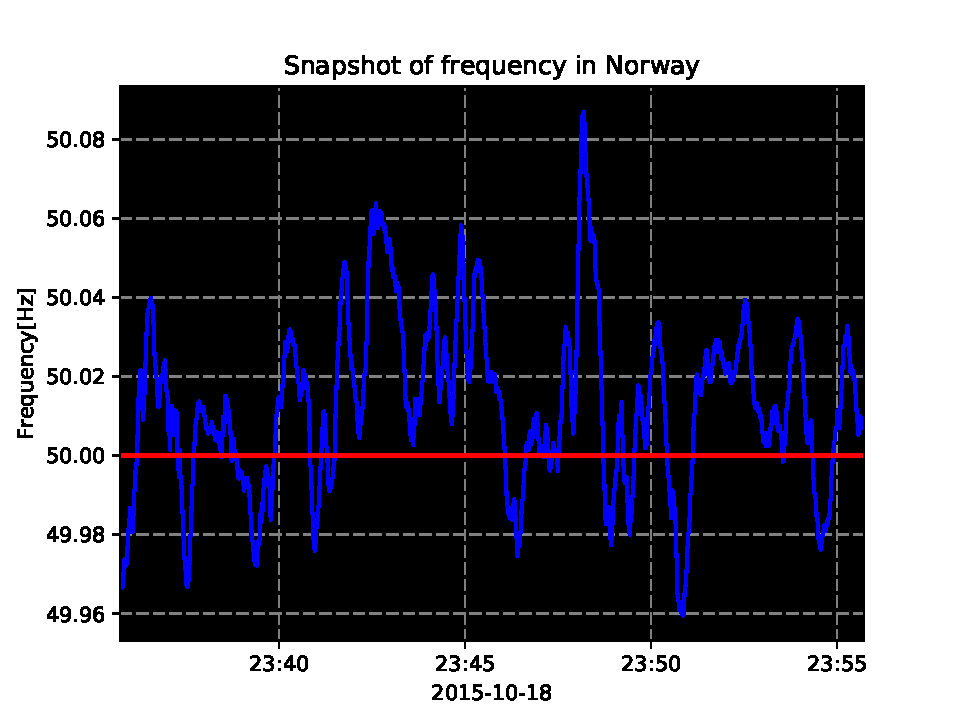
\includegraphics[width=0.8\textwidth]{./pictures/frequency.pdf}
			\end{figure}
		\end{column}
	\end{columns}
\end{frame}
\begin{frame}
	\frametitle{Challenges in operation}
	\begin{columns}
		\begin{column}{0.5\textwidth}
		\begin{itemize}
			\item<1-> Towards 100\% renewable electricity generation
			\begin{itemize}
				\item Larger variability
				\item More uncertainty
				\item Increasing complexity
			\end{itemize}
			\item<2-> More dynamics
			\item<3-> Less time for actions
			\item<4-> \textbf{Hydropower} is the main resource for balancing
\end{itemize}
\end{column}
	\begin{column}{0.5\textwidth}
		\begin{figure}
			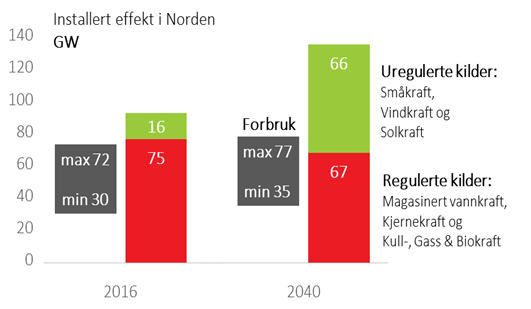
\includegraphics[width=0.8\textwidth]{./pictures/mix}
			\caption{Present and future energy mix[Statnett]}
		\end{figure}
	\end{column}
	\end{columns}
\end{frame}
\begin{frame}
	\frametitle{New requirements on FCR due to frequency quality}
	\begin{itemize}
		\item Nordic TSOs are developing new requirements on FCR
		\item This includes offline testing and verification of performance
		\begin{figure}
				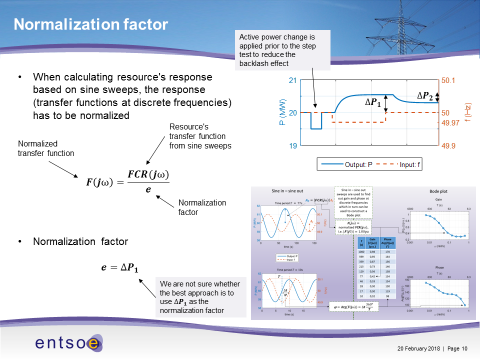
\includegraphics[width=0.4\textwidth]{./pictures/fcr}
		\end{figure}
	\end{itemize}
\end{frame}
\begin{frame}
	\frametitle{Theoretical background for new requirements}
	\begin{itemize}[<+->]
		\item Aggregated system model:
			\begin{itemize}[<+->]
					\item $G_{p_{sys}}(s)$: Aggregated model of FCR
					\item $G_{J_{sys}}(s)$: Aggregated model of swing dynamics
					\item $\Delta P_l(s)$: Aggregated load changes
			\end{itemize}
		\item Stability requirement stated in terms of the system's sensitivity function
				\begin{equation}
						S_{sys}(s) = \frac{1}{1+G_{p_{sys}}(s)G_{J_{sys}}(s)}
					\end{equation}
	\end{itemize}
			\begin{figure}
				\centering
				\includegraphics<1->{./pictures/req_sys.tikz}
			\end{figure}
\end{frame}
\begin{frame}
		\begin{columns}
			\begin{column}{0.6\textwidth}
					\begin{itemize}[<+->]
					\item Stability can be checked using:
						\begin{equation}
							L_{sys}(s) = G_{p_{sys}}(s)G_{J_{sys}}(s)
						\end{equation}
					\item Stability margin given by:
						\begin{equation}
								Ms = \min |-1 - L_{sys}(j\omega)|
						\end{equation}
					\item Notice that 
						\begin{equation}
								\min |-1 - L_{sys}(j\omega)| = \max|S_{sys}(j\omega)|
						\end{equation}
				\end{itemize}
			\end{column}
			\begin{column}{0.4\textwidth}
				\frametitle{Stability using Nyquist}
					\begin{figure}
						\includegraphics<1>[width=0.9\textwidth]{./pictures/nyquist_L_zoom_out.tikz}
						\includegraphics<2->[width=0.9\textwidth]{./pictures/nyquist_L.tikz}
					\end{figure}
				\end{column}
		\end{columns}
\end{frame}
\begin{frame}
	\frametitle{Draft requirements for performance}
	\begin{itemize}[<+->]
		\item For the performance we want to limit the change in frequency.
		\item The change in frequency is given by:
			\begin{equation}
				\Delta f_{sys}(s) = -2\pi G_{J_{sys}}(s)S_{sys}(s)d(s)=2\pi G_{1_{sys}}(s)d(s)
			\end{equation}
		\item We can use this for defining the performance requirements:
				\begin{equation}
						|2\pi G_{1_{sys}}(j\omega)|^2 \phi_d(\omega) < \phi_{\Delta f}(\omega) = 0.1
				\end{equation}
	\end{itemize}
			\begin{figure}
				\centering
				\includegraphics<1->{./pictures/req_sys.tikz}
			\end{figure}
\end{frame}
\begin{frame}
	\frametitle{Draft requirements for power plant}
	\begin{enumerate}[<+->]
			\item Measure a plant's response to ten sine injections
			\item Estimate $G_p^{(p.u.)}(s)$ for the plant based on the sine injections
			\item Use $G_p^{(p.u.)}(s)$ together with $G^{(p.u.)}_{J_{sys}}(s)$ to check.
				\begin{equation}
						|S(j\omega)| <\frac{1}{M_s}
				\end{equation}
				and
				\begin{equation}
						|2\pi G_{1}(j\omega)|^2 \phi_d(\omega) < 0.1
				\end{equation}
	\end{enumerate}
\end{frame}
\begin{frame}
	\frametitle{Drawbacks with the draft requirements}
		\begin{itemize}
			\item One has to disconnect the plant to inject the sine waves.
			\item Injecting  $10$ sine waves take a lot of time.
			\item They assume the same swing dynamics for all plants.
	\end{itemize}
	\end{frame}
\begin{frame}
	\frametitle{Research question}
	\begin{itemize}
		\item Can the draft requirements be tested using PMU measurements from normal operation?
	\end{itemize}
				\begin{equation}
						|S(j\omega)| <\frac{1}{M_s}
				\end{equation}
				and
				\begin{equation}
						|2\pi G_{1}(j\omega)|^2 \phi_d(\omega) < 0.1
				\end{equation}
	\begin{figure}
		\includegraphics<1>{./pictures/genTrafo.tikz}
	\end{figure}
\end{frame}
